\section{Introduction}

\section{Related Work}
Energy efficiency for constraint devices is a highly interest topic in the context of Internet of Things and can strongly impact on the quality of IoT services. For instance, in IOT agriculture scenario where IoT devices are widely distributed in a large region, optimizing the energy consumption may extend the device life circle as well as significantly reducing the maintenance cost.\\

Considering the fact that waking-up, collecting and pre-processing cost consume a small proportion of energy comparing with transmitting. Thus, energy could be saved by not transmitted unneeded samples, that is also the goal of adaptive sampling approach. The basic idea of adaptive sampling technique is to adapt the sampling rate to the change of observation based on certain criteria  while ensuring the precision  of outcome information []. In this section, we catalog the adaptive sampling approaches relied on such criteria.
\par \textit{Send-on-delta sampling}: is the most commonly used in wireless networks. The original of such approach is the level-crossing sampling at late 1950s based on the idea ``the most suitable sampling is by transmission of only significant data, as the new value obtained when the signal is changed by a given incremen'' \cite{ellis1959extension}. Due to its popularity, there are various temps expressing this strategy such as event-based sampling \cite{940692},  magnitude-driven sampling \cite{persson2001event} or deadbands \cite{otanez2002using}. Formally, given threshold $ \delta $, a message has value $ y_i $ at $ t_i $ is sent if and only if 
\begin{equation}\label{key}
(y_i - y_k) > \delta
\end{equation}
with $ y_k $ is the last message be sent at $ t_k $. To prevent babbling-idiot failure on such approach, the min and max sending time, denoted by $ T_L $ and $ T_H $ respectively, are defined as the boundary of sampling interval ($ T_L \leq t_i - t_l \leq T_H $)\\

\textit{Integral Sampling} uses the concept of integral or energy of the error to deal with small oscillations in the signal. The message is sent if the accumulated error of sampling, denoted by CES, is greater than a pre-defined threshold $ \xi $. The min and max-send-time are also applied. The CES value of a signal $ x(t) $ is the deference between $ x(t) $ and accumulated value from the most recent sample $ x(t_k) $. 
\begin{equation}\label{CES}
CES_{x_t} = \displaystyle\int\limits_{t_i}^{t_{i-1}} [x(t) - x(t_{t-1})]^{2}dt
\end{equation}
where $ i=1,2,...,n $ is the number of sample taken from $ t_0 $ to $ t_n $ \cite{miskowicz2005sampling}\\

\textit{Predictor-based sampling} uses a model to predict the next measure based on the past values. The message $ x(t) $ is sent if it significantly differs with  the predicted value $ \hat{x}(t) $. The criterion of the difference may reuse either sen-on-data or interval sampling. The model is build from a simplified statistic using linear extrapolation \cite{suh2007send}. To maintain the information quality, the predictor is also used in receiver to extrapolates the signal value until receiving the new message. However, updating receiver predictor requires at least 2 samples. This reduces the efficiency of such approach.\\

\textit{Gradient-based integral sampling} is an extension of integral sampling approach with the optimization of wake-up energy consumption. This method bases on the fact that waking-up device consumes considerably larger than collecting message. Thus, the next wake-up time is automatically adjusted to the current gradient of the signal \cite{ploennigs2009comparison}. To the avoid the worst scenario which the signal gradient is zero, a max-sleep-time is defined. \\

\textit{Sigmoid-based sampling} uses a sigmoid function to estimate the change of sampling rate based on the the variance of the last windowed signal \cite{shu2017energy} \cite{alippi2010adaptive}. Let denote the last message be $ x(t) $ belonging a signal window size $ W $, the variance is the absolute difference of between $ x(t) $ and $ x(t-1) $ over the average value of $ W $. Then such variance is compared with a pre-determined threshold before calculating the new sampling rate is the multiplication of current race and the sigmoid function of such variance. Such new rate is  changing rate is limited from 0 to 2 as a result of sigmoid function properties. 

%%%%%%%%%%%%%%%%%%%%%%%%%%%%%%%%%%%%%%%%%%%%%%%%%%%%%%%%%%%%%%%%%%%%%%%%%%%%%%%%%%%%%%%%%%%%%%%%%%%%%%%%%%%%%%%%%%%%%%%%%%%%%%%%%%%%%%%%%%%%%%%%%%%%%%%%%%%%%%%%%%%%%%%%%%%%%%%%%%%%%%%%%%%%%%%%%%%%%%%%%%%%%%%%%%%%%%
\section{Adaptive Sampling Algorithm}
Unlike the existing adaptive sampling algorithms that share a vulnerability to configuration parameters, we propose a light-weight adaptive frequency for improving the power efficiency based on user's desire while maximizing the sampled data. In this section, we first present the overall algorithm. Then, we briefly explain each step along with related definitions.

\subsection{Preliminaries}
\textbf{Definition 1}(Absolute first difference). The absolute value of first difference of $ \theta_{i}(p) $, denoted as $ \triangle\theta_i(p) $, which is defined that:
\begin{equation}\label{First_difference}
\triangle\theta_i(p) = |\theta_{i}(p) - \theta_{i-1}(p)|,\, i = 1, 2, 3, ..., n
\end{equation}

\textbf{Definition 2}(Absolute Second difference). The absolute value of second difference of  $ \theta_{i}(p) $, denoted as $ \triangle " \theta_i(p) $, which is defined that:
\begin{equation}\label{Second_difference}
\triangle"\theta_i(p) = |\triangle\theta_{i}(p) - \triangle\theta_{i-1}(p)|,\, i = 1, 2, 3, ..., n
\end{equation}

\subsection{Overview Algorithm}
The light-weigh adaptive sampling algorithm is designed to optimize power utilization of constrained devices in IoT. Given the desire power saving level, the algorithm maximize the accuracy of sample data at such level.  \\

The general idea of our proposed algorithm is to dynamically adapt the sampling frequency according to the observation changes. Obviously, a higher frequency is strongly preferred to context awareness when there are significant changes in the observation. For example, in forest fire warning service, the sudden increase of temperature is considered as notable events. Increasing frequency may help to deeper investigating such events. In contrast, if the observed value is hardly fluctuate, a decrease in frequency is desired to save energy in data sampling, processing and transmission. \\

To archive these assumptions, a enhanced sigmoid function is exploited to quickly adapt the sampling frequency, which is described as: 
\begin{equation}\label{Fchange}
 f_{change} = n + \frac{1-n}{1 + e^{-n*D}}
\end{equation}
with:
\begin{equation}\label{D}
 D = \frac{\triangle\theta_i(X_i) - \frac{n+1}{2}*(\frac{1}{N}\sum_{j=i-N}^{i} \triangle\theta_i(X_j))}{\frac{1}{N}\sum_{j=i-N}^{i} \triangle\theta_i(X_j)}
\end{equation}

In the equation \ref{Fchange}, n is the user desire of power saving; and D presents the sudden change of coming data comparing with sliding window based N most recent data. It is reasonable to compare the change of 
the absolute difference between $ X_i $'s absolute first difference over the mean value of such difference of last N data points. If D is sufficiently large, this means the current change is overwhelming in comparison with recent history. Then the sampling frequency is adapted with this change. In contrast, if the value of D is negative, which means the values change is not large enough, the sampling frequency can be reduced to save the device resources. \\

As the result of extended sigmoid function, the theoretical value of new frequency is limit in a certain range from standard frequency (assuming to equal 1) to user desire (n), that is, regardless the value of D, new frequency denoted by y(D) is always in defined boundary. This barrier is vital in constrained network such as LPWAN, SIGFOX whereas the boundary of sending messages interval is strictly limited. The presentation of y(D) function is illustrated in figure 1. It is found that the value of y is highly change when the D value is in range from -1 to 1,that is, change of lasted sampled data is higher from $ \frac{n-1}{2} $ to $ \frac{n+3}{2} $ times than the mean of this change in history. For the rest value of D, the y(D) converges to border of its boundary. Hence, the new sampling frequency for the next iteration is capable of adapting to change in lasted data and bounded in desired ranges, which satisfy the needs for a effective frequency algorithm as well as energy conservation. \\

Our proposed algorithm manipulates the extended sigmoid function corresponding with natural sampling process which is robust with faulty in sensed data. This scheme ensures that the new frequency is calculated not only based on lasted sensed data but also historical data which presents the overall data trend. In more detail, a anomaly value in sensor reading, which may be significantly higher than the average change recently, does not strongly impact on the next sampling frequency. The frequency only significantly changes when there are consecutive changes in obtained data. As the result, our approach effectively determine whether the device energy is either consumed or conserved based on the trend of the sensed data rather than uncertain changes on last value. 
The pseudo code for implement our proposal is presented as below:


\begin{table}[h]
	\centering
	\begin{tabular}{l}
		\toprule
		\textbf{Algorithm 1:} Adaptive Frequency for of newest data point $ X_i $\\
		\midrule
		\textbf{Input: } $ X_i $, window size $ N = 50 $ \\
		\textbf{Output:} New frequency $ f_{new} $ \\
		1.~ Initializing: Window W = \{$ X_{i-N}, X_{i-N+1}, .... , X_i $\}	 \\
		2.~ Calculating changing degree: \\
		\hspace{10mm}		$ D = \frac{\triangle\theta_i(X_i) - \frac{n+1}{2}*(\frac{1}{N}\sum_{j=i-N}^{i} \triangle\theta_i(X_j))}{\frac{1}{N}\sum_{j=i-N}^{i} \triangle\theta_i(X_j)} $ \\
		3.~ Calculating the new frequency: \\
		\hspace{10mm} 		$ f_{new} = n + \frac{1-n}{1 + e^{-n*D}} $\\
		\textbf{return $ f_{new} $}
	\end{tabular}
	\label{tab:AL_1}
\end{table}


\section{Experimental Evaluation}
In this section, we present the evaluation result to demonstrate the efficiency of our proposal on both real and synthetic dataset. We also experimentally compare with the common anomaly detection approaches using NAB \cite{lavin2015evaluating}. At the end, we discuss the importance of Active learning in CABD.
%In this section, we empirically evaluate the quality and efficiency of our proposal on both real and synthetic dataset. We demonstrate that:
%\begin{itemize}
%	\item CABD effectively detect both single and collective anomalies which need to be removed.
%	\item CABD quickly identify the key deviation event which also known as break point.  
%	\item Applying active learning significantly improves the CABD’s accuracy. 
%\end{itemize}
%We briefly describe each of these goals below

%\subsection{User studies}
%\subsubsection{User study 1: Tank Monitoring}
%\subsubsection{User study 2: Humility Monitoring}


\subsection{Metric of Measurement}
For evaluating the efficiency of proposed algorithm, we use two metric:
\begin{itemize}
\item Normalized Mean Error (NME) to indicate the overall goodness of fit after normalizing between the original signal and reconstructed signal from sampled data. This factor is defined as:
\begin{equation}\label{NME}
NME = \frac{1}{n}\sum_{i=1}^{n} |\hat{x}_i - x_i | * 100\%
\end{equation}
with $ \hat{x}_i $ denotes the normalized \textit{i}th data in the reconstructed signal, $ x_i $ represents the normalized \textit{i}th data in the original signal and n is the size of signal.
\item Resource Saving Factor (RSF) to indicate the conserved resources based on the reduce in transmitted messages be defined as: 
\begin{equation}\label{RSF}
RSF = \frac{\hat{m}}{n}
\end{equation}
with m and n are the size of sampled data and original data respectively.
\end{itemize}
  
\subsection{Benchmark Datasets}
\textit{National Oceanic and Atmospheric Administration (NOAA) datasets: } The NOAA provides a set of real-time data about water-quality from a place named "Jamestown". In order to reasonably compare with state-of-the-art approaches, we choose the same dataset and monitoring duration ranges with them which are turbidity and DO from 15 December 2016 to 15 March 2017. \\

\textit{IoT datasets: } The data is collected from 2 real CO2 sensors deployed in the working space with the sampling interval of 1h for a sample. 

\subsection{Evaluative Simulation}

To assess our proposal performance, we simulate the evaluation process closing with real deployment on device. First, the initial sampling frequency is set to the original frequency of dataset. Then the next sampling is calculated by the algorithm. We derive the data value for this sampling from original dataset by using a linear interpolation method. The process is repeated until the next sampling is out of original dataset. The new obtained dataset by our method is up-sampled to the size with original dataset  and normalized before calculating the metric of measurement. The process is presented in the algorithm 2. \\
\begin{table}[h]
	\centering
	\begin{tabular}{l}
		\toprule
		\textbf{Algorithm 2:} Evaluation Process\\
		\midrule
		\textbf{Input: } Dataset X, Window size N, Saving desire n \\
		\textbf{Output:} $ NME, RFS $ \\
		1.~ $ f_{curr} \leftarrow f_{const}$   \\
		2.~ Y = [ $ X_0, X_i, ...., X_n $ ], i = N \\
		3.~ \textbf{While} $ i < size(X) $ \textbf{do} \\
		\hspace{10mm}$
		\left \|  
		\begin{tabular}{l}
		$ f_{new} \leftarrow $ MyAL($ Y, N ,n $) \\
		$ X_{next} \leftarrow $ Interpolation($ X, f_{new} $)\\
		$ f_{curr} \leftarrow f_{new} $\\
		$ Y = Y \cup \{X_{next}\} $\\
		$ i = i + \frac{1}{f_{new}} $\\
		
		\end{tabular}
		\right .
		$\\
		4.~ $ \hat{X} \leftarrow UpSample(Y) $  \\
		\hspace{5mm}$ \hat{X}_{norm} \leftarrow Normalize(\hat{X}) $  \\
		\hspace{5mm}$ X_{norm} \leftarrow Normalize(X) $  \\
		\textbf{Return $ NME(X_{norm}, \hat{X}_{norm}),  RSF(Y,X) $}
		
	\end{tabular}
\end{table}

\subsection{Results}

\subsubsection{Varying user desire n}

\begin{figure*}[h]
	\centering
	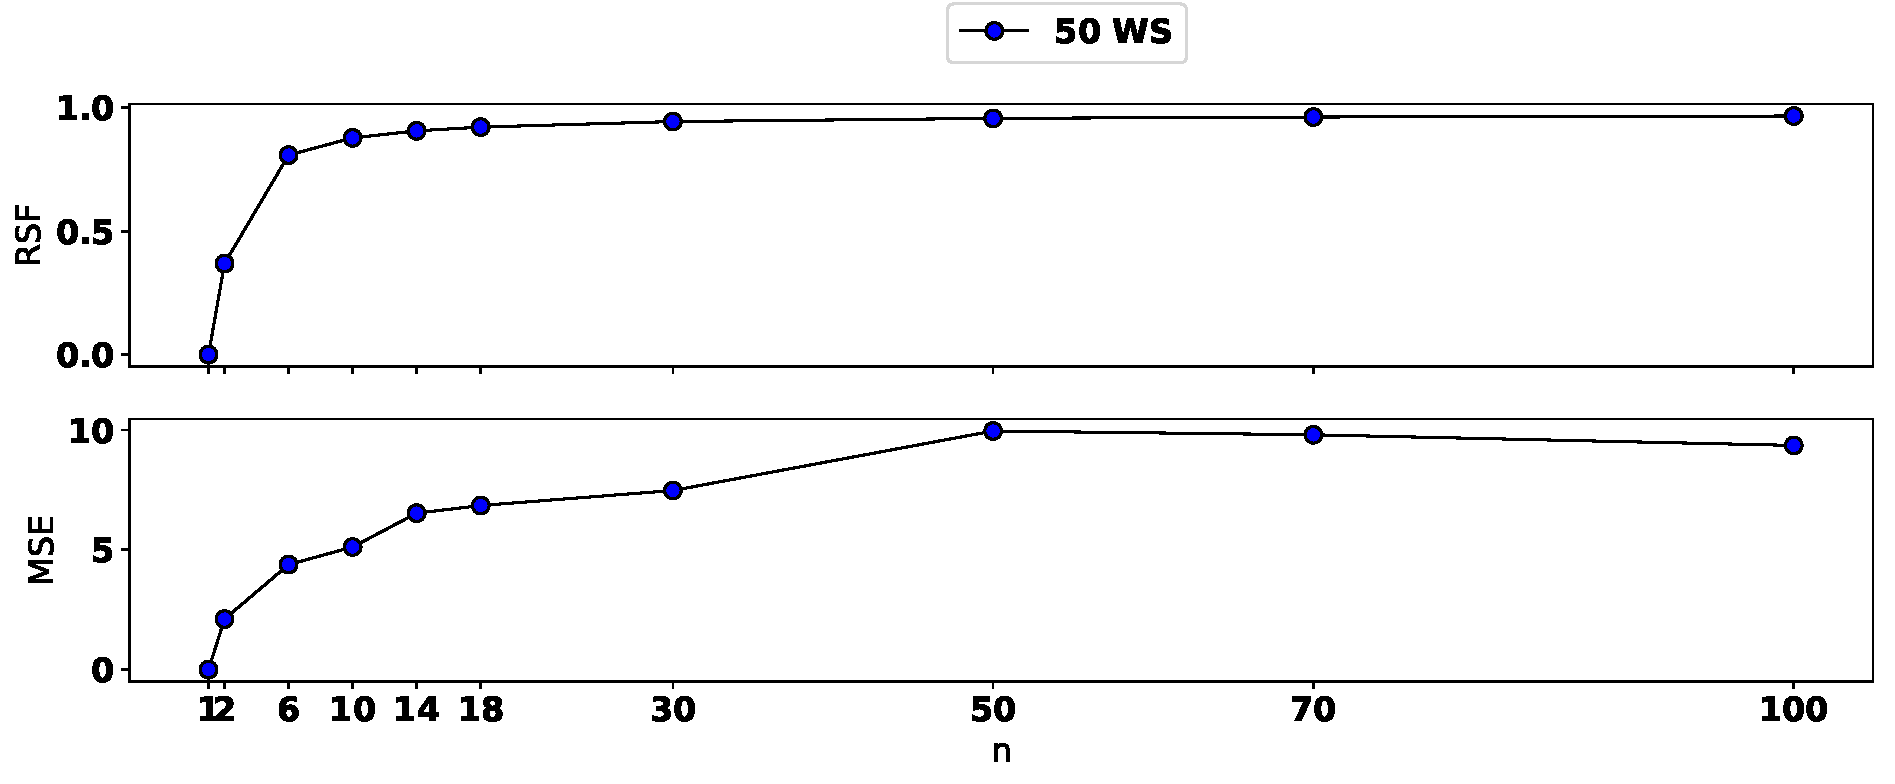
\includegraphics[width=0.95\textwidth]{Part3/Chapter8/figures/result_various_n.pdf}
	\caption{ : Varying user desire n, over DO dataset with window size = 50.}
	\label{fig: various_n}
\end{figure*}

Figure \ref{fig: various_n} present the result on varying user desire n, for DO database with fix window size equals 50. First, as shown in figure \ref{fig: various_n} (a), our proposal shows better resource saving with the increase of user desire n. This means more saving desire leads to less transmitted message. Setting n to 1 leads to the new frequency always equals the origin frequency. As a result, the RSF value equals 0 due to no saving resource. 
Remarkably, the RSF value increase at low n value from 1 to 6 but it slightly coverages to a stable level. This happens mainly because the n value is considered as the upper asymptote of the frequency and does not strongly impact on the algorithm output. At an sufficient large n, the RSF value will be stable. \\%The similar result are also observed in real IoT dataset. \\

\begin{figure*}[h]
	\centering
	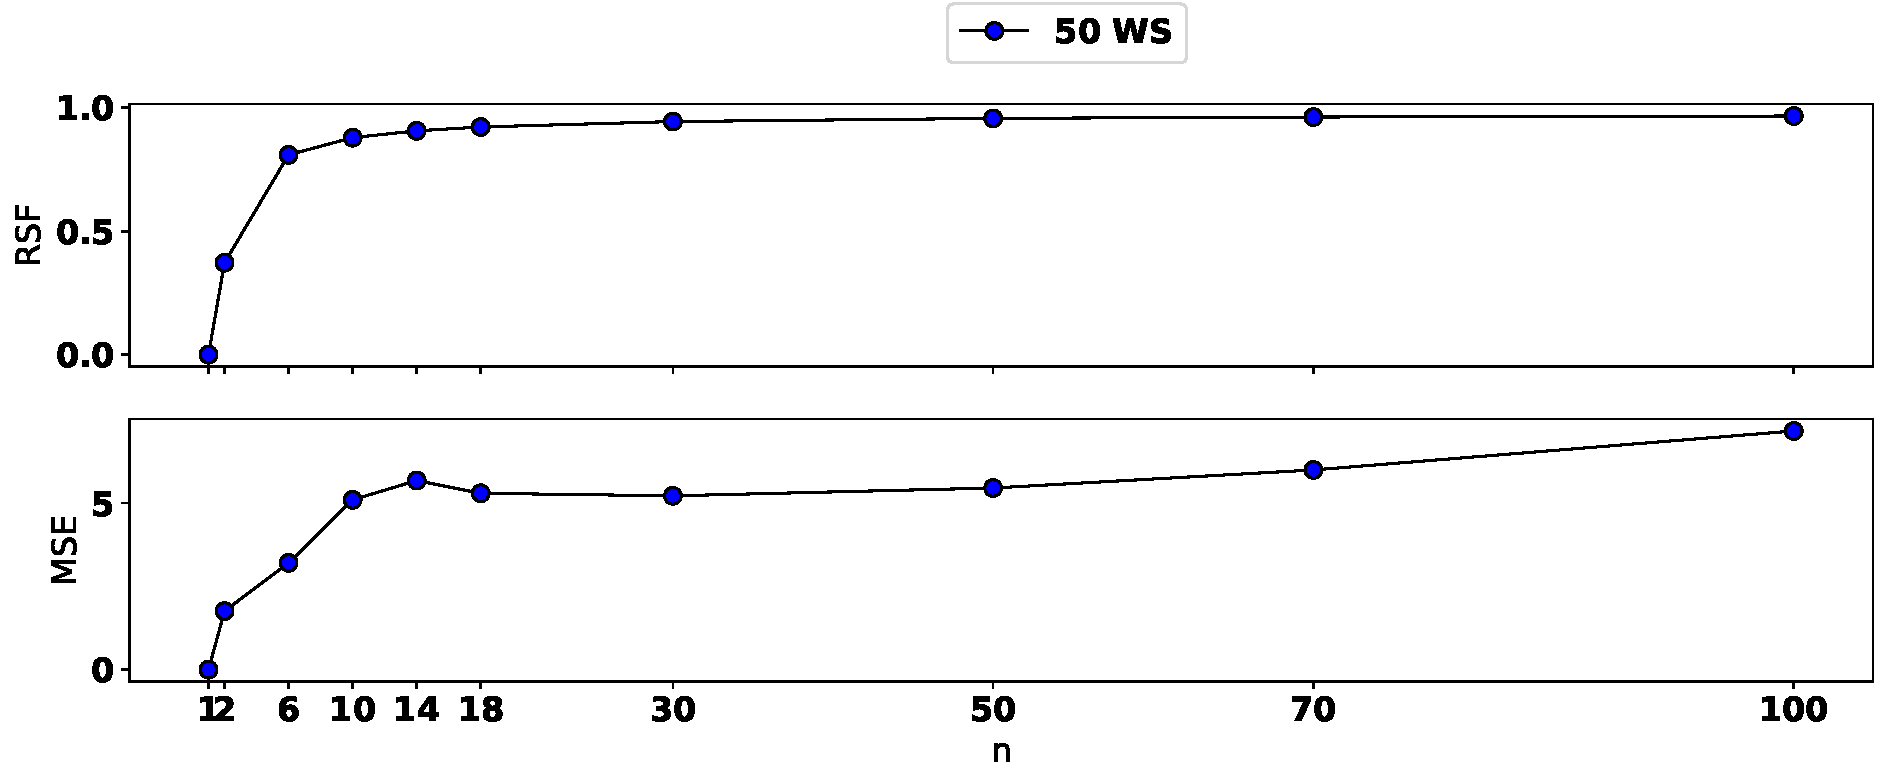
\includegraphics[width=0.9\textwidth]{Part3/Chapter8/figures/result_various_n_iot.pdf}
	\caption{ : Varying user desire n, over DO dataset with window size = 50.}
	\label{fig: various_n_iot}
\end{figure*}

It is not surprising that the change of MSE and RFS is similar while increasing n value. This is illustrated in figure \ref{fig: various_n} (b) wherein the MSE value is significant increase from 0 to 5 with the increase of n from 1 to 6 then it slowly coverage to stable value, since the MSE is proportional to RFS. This could be explained that higher RFS means less data is sampled and transmitted. Therefore, the reconstructed data is more different with original data. This leads to the increase of MSE. \\
In summary, as presented in Figure \ref{fig: various_n} and \ref{fig: various_n_iot} over the DO and temperature datasets, our proposal is capable of not only preserving the device's resources based on user desire but also being robust with excessively large desired configuration. 

\subsubsection{Varying window size N}

\begin{figure*}[h]
	\centering
	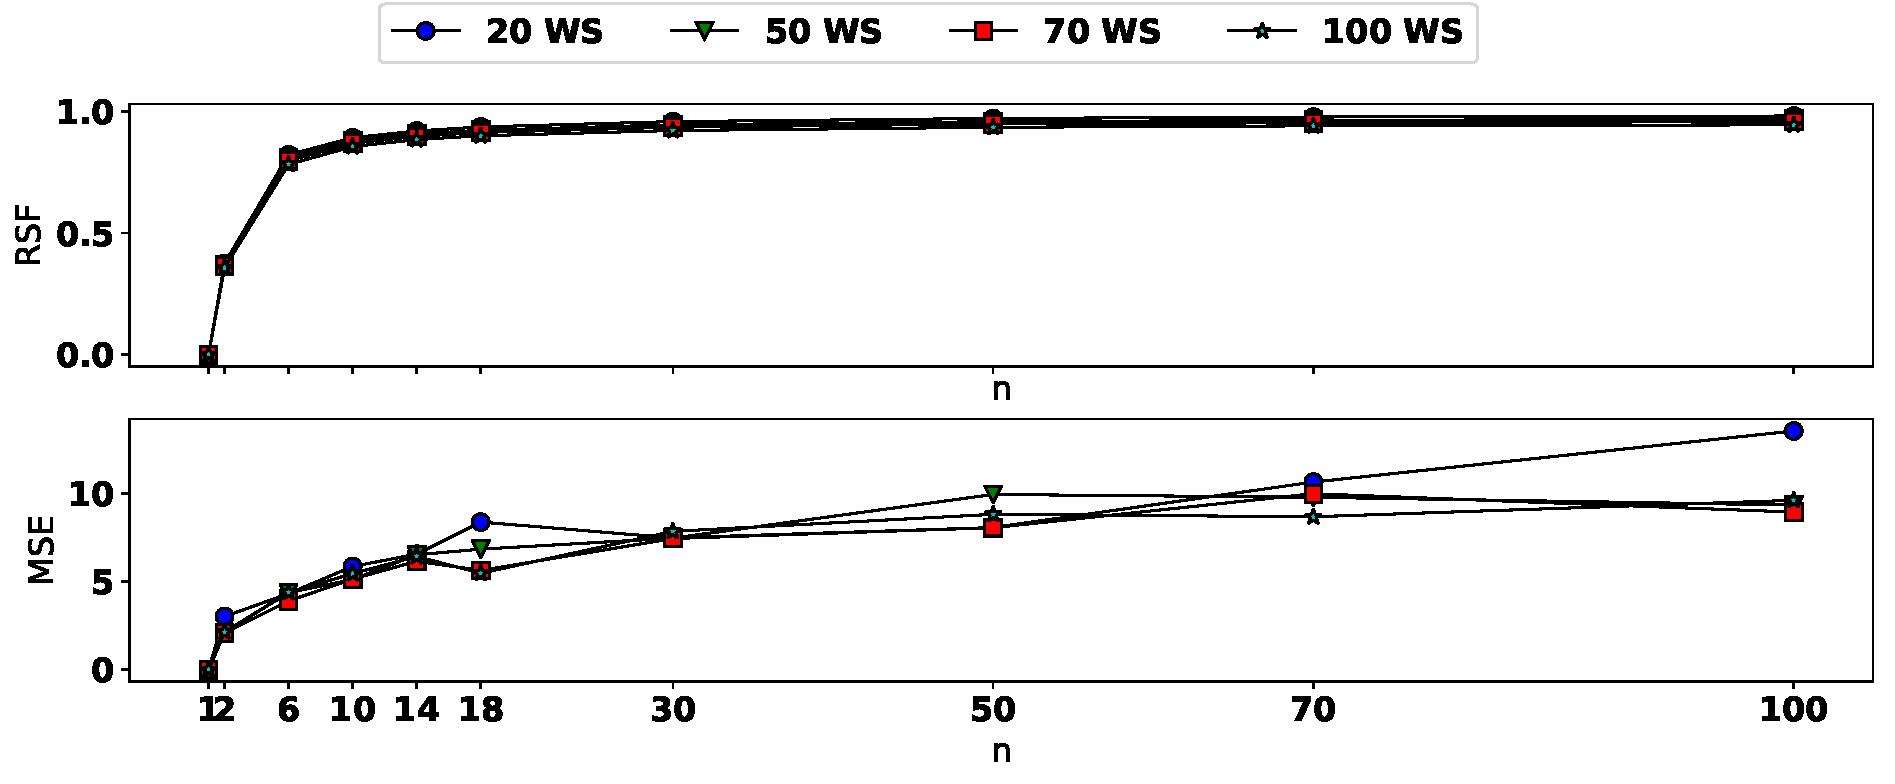
\includegraphics[width=0.9\textwidth]{Part3/Chapter8/figures/result_various_windowsize.pdf}
	\caption{ : Varying user desire n, over DO dataset with window size = 50.}
	\label{fig: various_ws}
\end{figure*}

Figure \ref{fig: various_ws} reports the result by varying the window size ws for different n value on DO dataset. As illustrated, we note that both the RSF and MSE value is independent with ws configuration. While increase the window size from 20 to 100, the RSF is stable around a constant value. For example:......... This results from the superiority of D function. In more detail, the D function compares the current changes degree with the mean of first derivate of historical data. By increasing window size to obtain more history does not strongly impact on this mean, that is, the optimized frequency is well-balanced with the increase of window size. The similar result for Turnity dataset is presented in figure \ref{fig: various_ws_iot}. This result again consolidates the effectiveness and consistency of our algorithm.

\begin{figure*}[h]
	\centering
	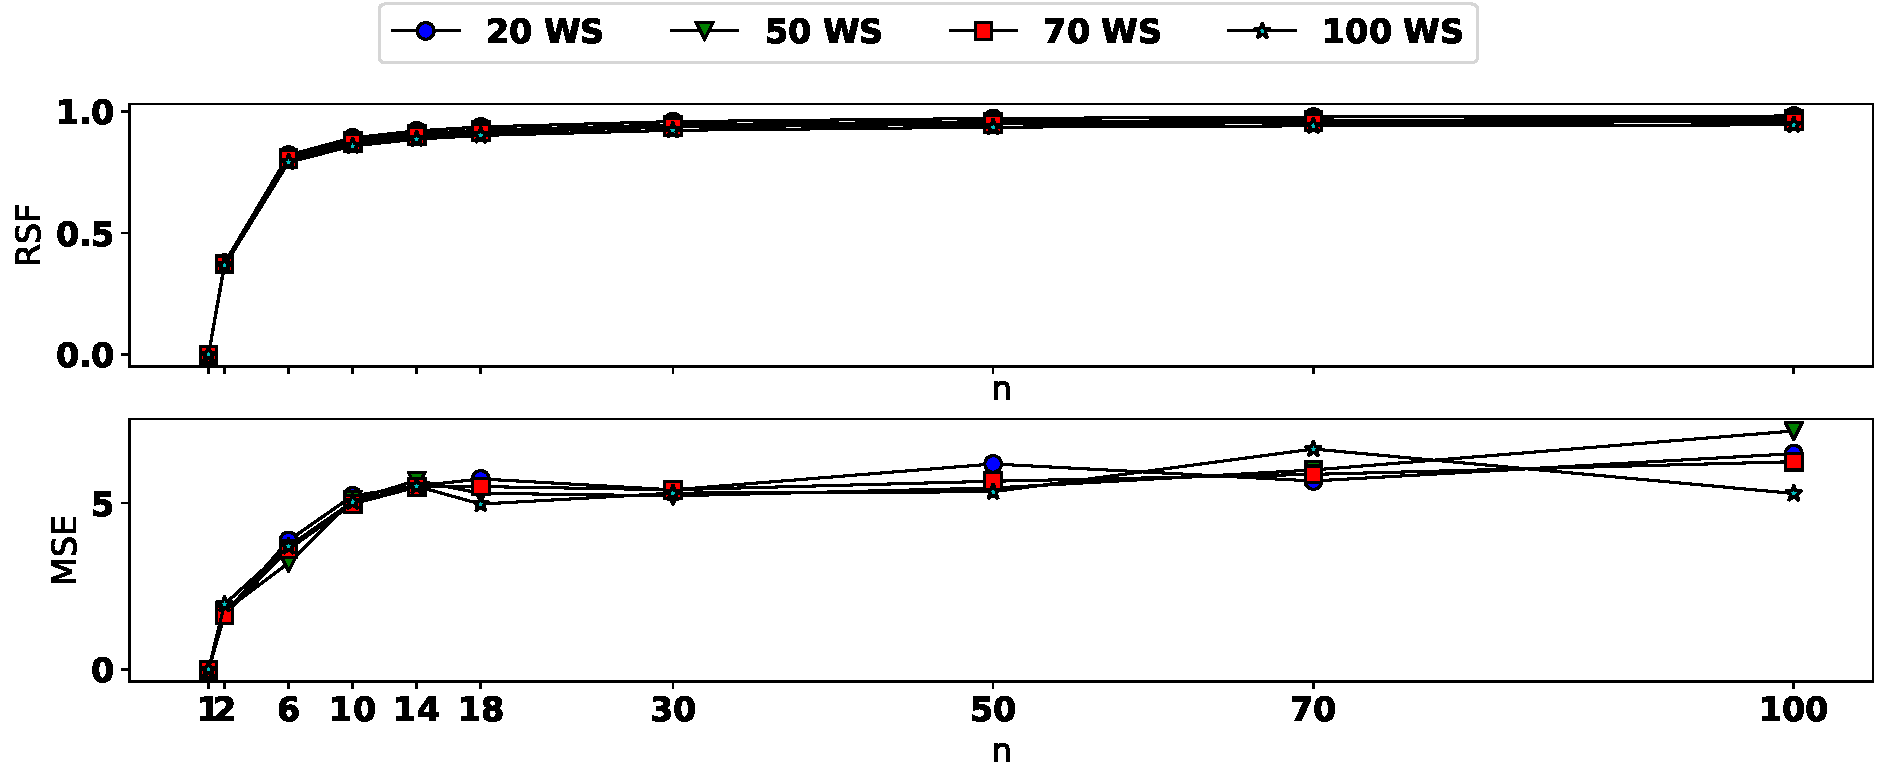
\includegraphics[width=0.9\textwidth]{Part3/Chapter8/figures/result_various_windowsize_iot.pdf}
	\caption{ : Varying user desire n, over DO dataset with window size = 50.}
	\label{fig: various_ws_iot}
\end{figure*}

\subsection{Comparison of Results}
We do state-of-the-art a number of adapting sampling algorithm for saving energy but evaluating all of them is extremely heavy. Hence, the compared algorithms are DDASA \cite{shu2017energy}, ASA \cite{alippi2010adaptive} which are the most related with our approach. For transparency, The competitor results are derived from original paper. In order to obtain NME value with the sample size of these results, we execute our algorithm with various user desire value. The estimated NME is calculated by interpolation method.\\

A comparative analysis of NME on DO dataset is presented in table \ref{tab: performance comaprison}. Considering the fact that larger number of sample will definitely consume more energy to collect, store and transmit data. As illustrated, our proposal shows superiority  over the competitors in case of high saving energy. To reduce original dataset to 297 and 421 samples,  the NME values of our approach are around 4.96\% and 4.07\% in comparison with 9.99\% and 8.43 \% of DDASA respectively. This means that the reconstructed data from our selective points is more likely to original data than others. Moreover, our approach is more consistent and robust than the competitor while dealing with high power saving scenario. This is demonstrated by the minor change of NME while reducing the number of sample. In more detail, our NME variance is around 0.79 comparing with 13.6 of DDASA while decrease the sample size from 1064 to 297.\\

In summary, comparing with other approaches, our algorithm has better performance which is demonstrated by lower and more consistent in MSE value. 
%\begin{table*}[h]
%	\centering
%\begin{tabular}{l*{6}{c}r}
%	              & DDASA & DDASA & DDASA & DDASA & ASA & DDASA &Fixed Rate   \\
%	              & (t=0.07) & (t=0.03) & (t=0.02) & (t=0.015) & & (t=0.01)& Sampling  \\
%	\hline
%	Number of Samples & 146 & 297 & 421 & 548 & 637 & 1064 & 2182   \\
%	NME            & 11.7 \% & 9.99 \% & 8.43 \% & 5.31 \% & 5.52 \% & 1.62 \%&  0   \\
%	AFO NME         &7.16 \%& 4.96  \%&  4.07 \% &  4.37 \% &  3.86 \% & 2.84 \%&  0\\
%\end{tabular}
%		\caption{: Performance comparison.}
%\label{tab:gcz_data_synthetic}%
%\end{table*}%

\begin{table*}[h]
	\centering
	\begin{tabular}{l*{6}{c}r}
		&  & DDASA & DDASA & DDASA & ASA & DDASA &Fixed Rate   \\
		&  & (t=0.03) & (t=0.02) & (t=0.015) & & (t=0.01)& Sampling  \\
		\hline
		Number of Samples &  & 297 & 421 & 548 & 637 & 1064 & 2182   \\
		Competitor's NME            &   & 9.99 \% & 8.43 \% & 5.31 \% & 5.52 \% & 1.62 \%&  0   \\
		AFO NME         & & 4.96  \%&  4.07 \% &  4.37 \% &  3.86 \% & 2.84 \%&  0\\
	\end{tabular}
	\caption{: Performance comparison.}
	\label{tab: performance comaprison}%
\end{table*}%

\section{Conclusion}
